\chapter{Progettazione}

\section{Progettazione MDSP}
\subsection{Messaggi}


Le componenti del sistema che si trovano su elaboratori differenti comunicano tra loro per meggo di 'messaggi'. Tali messaggi rappresentano una particolare richiesta di servizi, oppure una corrispondente risposta.

Un messaggio possiede una 'tipologia' e un certo numero di 'argomenti', dipendenti dal tipo di messaggio.

Il tipico messaggio è composto da un header di 8 byte, cosi' suddivisi:



\begin{itemize}
\item 3 byte per la stringa MDC

\item 1 byte per la versione del protocollo

\item 4 byte per il tipo di messaggio
\end{itemize}

I messaggi possono avere un singolo parametro, oppure molti. Per 'parametro' qui ci si riferisce al parametro del messaggio, ovvero una stringa null-terminated, che a sua volta può contenere uno o più parametri a livello applicativo.






\subsubsection{LIST}
%
LIST

Composizione:

\begin{itemize}
\item header MDC
\item null-terminated string
\end{itemize}

la stringa può contenere una espressione regolare per la definizione del nome del
flusso ricercato


\subsubsection{ALST}
%
Answer LiST

Lista di parametri

\subsubsection{SREQ}
%
Stream REQuest

Singolo parametro

\begin{itemize}
\item hash dello stream
\end{itemize}

\subsubsection{ASRQ}
%
Answer Stream ReQuest

Singolo parametro

\subsubsection{SINF}
Stream INFormation

Singolo parametro

\subsubsection{ASNF}
%
Answer Stream iNFormation

Singolo parametro

\subsubsection{PARM}
%
PARaMeters

\subsubsection{KALV}
%
Keep ALiVe

Singolo parametro

\subsubsection{PEER}
%
PEER

Singolo parametro

\subsubsection{APER}
%
Answer PEeR

Lista di parametri

\subsection{Descrittore}


Un 'Descriptor' è, nell'ambito di questo sistema, una unità di dati di un flusso multimediale.

Il flusso multimediale è suddiviso in sotto-flussi detti 'descrizioni', secondo le specifiche della codifica md; ogni descrizione è composta da un certo numero di descrittori, con la stessa relazione che c'è tra un filmato e un fotogramma.

Il Descriptor contiene varie informazioni, come il flusso originario, il numero di descrizione, e la sequenza temporale. Il payload non è definito e pertanto è permessa una maggiore libertà in fase di definizione dei codec.







\section{Codec}
\label{cap:descrizione_codec}
Il paradigma di protocollo di streaming a descrittori multipli rende
necessaria la progettazione di codec su misura. Viene rimandata al capitolo
\ref{cap:implementazione_codec} la presentazione, a titolo esplicativo, del
\emph{codec testuale}.

\subsection{Caratteristiche del codec}
Affinché un codec possa funzionare con il protocollo MDC (\emph{Multiple
Description Coding}) è necessario che possieda delle caratteristiche ben
precise. La codifica MDC ha come obiettivo finale la descrizione di un file in
modo tale che, in caso di perdita parziale dei dati che lo costituiscono, il
file stesso sia ugualmente interpretabile. L'assoluta interpretabilità del
file costituisce un vincolo molto stringente e si rendono necessari codec
progettati con particolari accorgimenti. MDSP versione 0.1 gestisce file di
tipo testuale e immagini, consente di visualizzare il contenuto di un file anche
se si verificano errori nel trasferimento dello stesso attraverso una rete di telecomunicazione. Durante la fase di codifica il file sorgente viene suddiviso in descrizioni e descrittori:
\begin{itemize}
 \item Un descrittore è la più piccola unità di misura del contenuto di un
 file. L'insieme di più descrittori costituisce una descrizione.
 \item Una descrizione può contenere parte o tutte le informazioni di un file
 (con `informazioni' si intendono i dati costituenti il file).
\end{itemize}
Le descrizioni costituiscono differenti codifiche e devono essere il più possibile ortogonali fra loro, in modo da poter essere indipendenti l'una dall'altra, pur riferendosi tutte allo stesso file sorgente.

Nel caso in cui qualche descrizione venga persa, sia corrotta, o non venga
inviata dalla sorgente, sarà comunque possibile decodificare il file ed
otterene un output sufficientemente corretto, tale da poter essere intepretato. \`E sufficiente la ricezione di una sola descrizione per la corretta ricostruzione del file sorgente. La ricezione di due o più descrizioni migliora l'accuratezza del file decodificato. Il file sorgente viene `\emph{descritto}' con più precisione.  Tale risultato viene raggiunto grazie alla creazione di codec che tengono in considerazione il fattore umano nell'interpretazione di vari tipi di informazioni:
\begin{itemize}
 \item Nel caso del testo, una parola con una lettera mancante viene facilmente interpretata dal lettore. Il cervello umano sostituisce la lettera mancante con quella corretta basandosi sul senso della parola stessa o della frase.
 \item Nel caso delle immagini, la mancanza di pixel non rende l'immagine inutilizzabile. All'occhio umano saranno presenti delle lievi alterazioni, ma, anche questa volta, il contesto rende ugualmente interpretabile l'immagine e le informazioni che essa contiene.
\end{itemize}

\begin{figure}[ht]
\centering 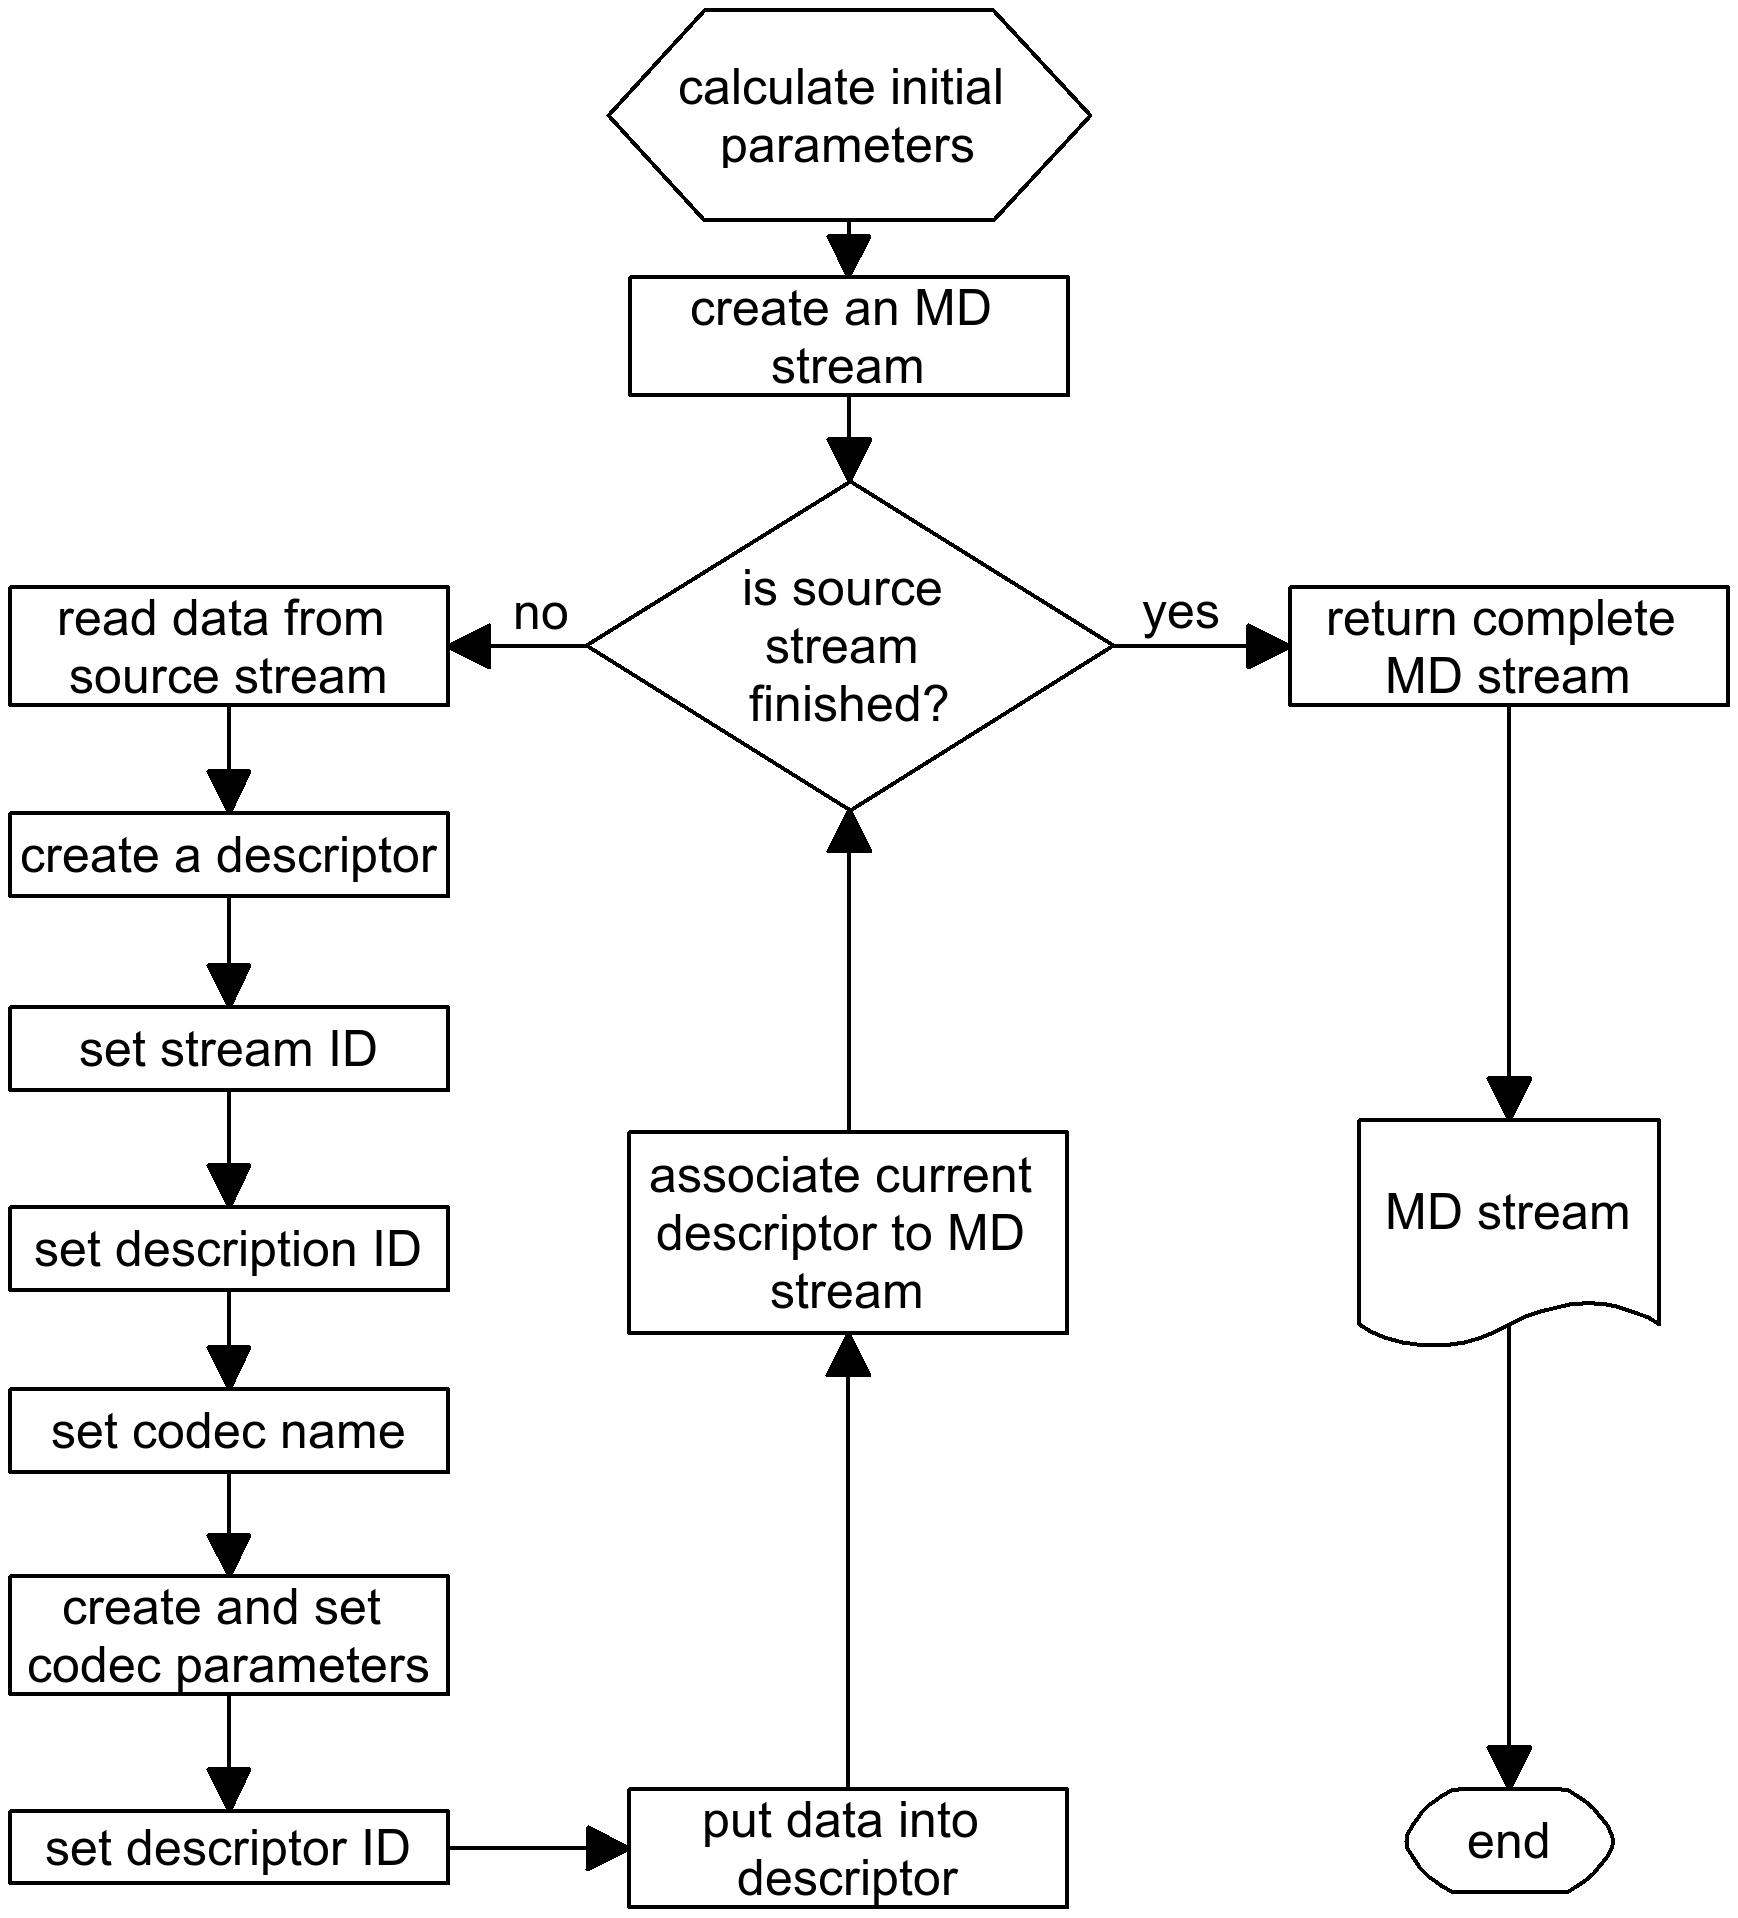
\includegraphics[width=0.90\textwidth]{../images/codifica.png}
	\caption{Diagramma di flusso dell'algoritmo di codifica.}
	\label{fig:codifica}
\end{figure}

\begin{figure}[ht]
\centering 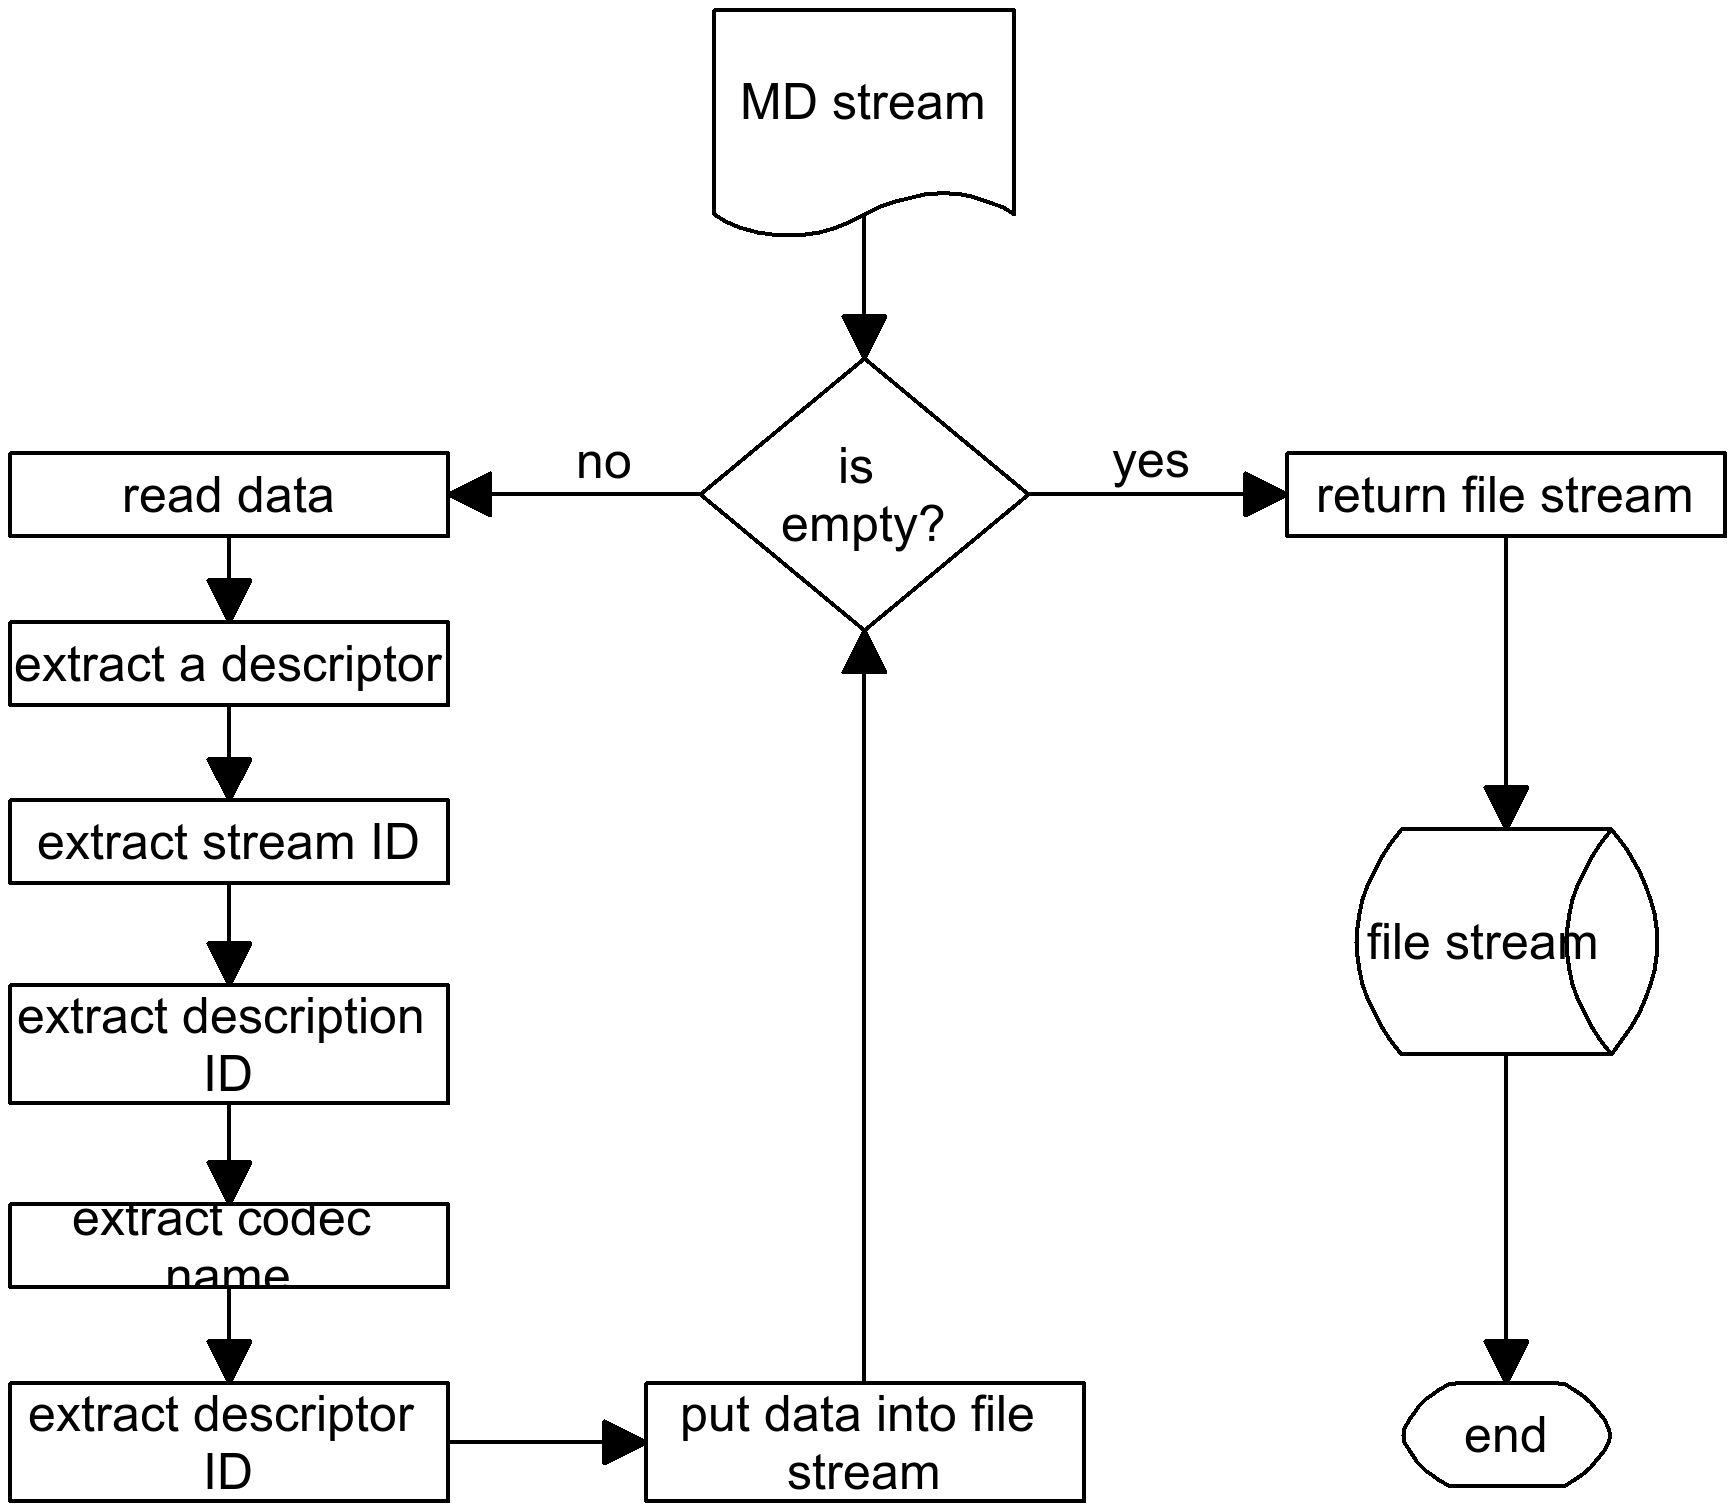
\includegraphics[width=0.90\textwidth]{../images/decodifica.png}
	\caption{Diagramma di flusso dell'algoritmo di decodifica.}
	\label{fig:decodifica}
\end{figure}

Il funzionamento del codec (illustrato in figura \ref{fig:codifica} e
\ref{fig:decodifica}) si può applicare per descrivere la suddivisione di ogni
descrizione in descrittori. Come accennato, i descrittori sono la più piccola unità di memorizzazione dei dati costituenti il file sorgente. Tale
affermazione significa che, se viene perso un descrittore durante il
trasferimento, oppure i suoi dati non sono corretti, esso può essere
semplicemente non considerato. Ciò permette un'estrema flessibilità di
decodifica. Sostanzialmente, il decodificatore deve adattarsi alla tipologia e
quantità di dati collezionati e creare un file di output. Tale file sarà perfetto se non si sono verificate perdite, o ugualmente interpretabile in presenza di perdite.
